% Generated by LitigCharts.PublicationFigures. Captions and provenance are sidecars.
\documentclass[10pt,tikz,border=5pt]{standalone}
\usepackage{lmodern}
\usetikzlibrary{patterns,patterns.meta}
\begin{document}
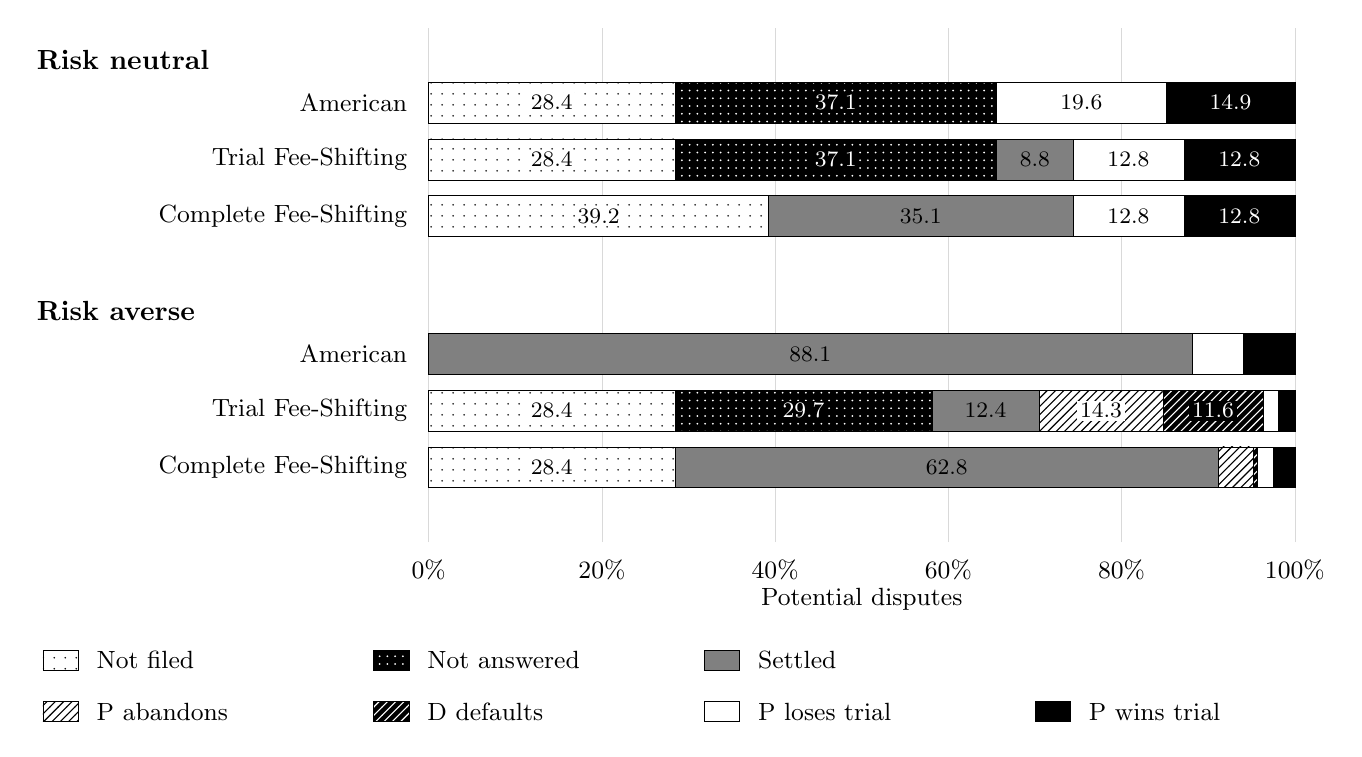
\begin{tikzpicture}[font=\small]\draw[black!15,line width=.2pt] (5.1,.65) -- (5.1,7.18);
\node[anchor=north] at (5.1,.55) {0\%};
\draw[black!15,line width=.2pt] (7.3,.65) -- (7.3,7.18);
\node[anchor=north] at (7.3,.55) {20\%};
\draw[black!15,line width=.2pt] (9.5,.65) -- (9.5,7.18);
\node[anchor=north] at (9.5,.55) {40\%};
\draw[black!15,line width=.2pt] (11.7,.65) -- (11.7,7.18);
\node[anchor=north] at (11.7,.55) {60\%};
\draw[black!15,line width=.2pt] (13.9,.65) -- (13.9,7.18);
\node[anchor=north] at (13.9,.55) {80\%};
\draw[black!15,line width=.2pt] (16.1,.65) -- (16.1,7.18);
\node[anchor=north] at (16.1,.55) {100\%};
\node[anchor=west,font=\bfseries] at (0,6.78) {\mbox{Risk} \mbox{neutral}};
\node[anchor=east] at (4.95,6.23) {American};
\path[preaction={fill=white,draw=none},pattern={Dots[distance=4pt,radius=.35pt]},pattern color=black,draw=black,line width=.25pt] (5.1,5.97) rectangle (8.22741,6.49);
\node[text=black,fill=white,font=\footnotesize,inner sep=1pt] at (6.663705,6.23) {28.4};
\path[preaction={fill=black,draw=none},pattern={Dots[distance=2.8pt,radius=.35pt]},pattern color=white,draw=black,line width=.25pt] (8.22741,5.97) rectangle (12.312766,6.49);
\node[text=white,fill=black,font=\footnotesize,inner sep=1pt] at (10.270088,6.23) {37.1};
\path[fill=white,draw=black,line width=.25pt] (12.312766,5.97) rectangle (14.464685,6.49);
\node[text=black,fill=none,font=\footnotesize,inner sep=1pt] at (13.388726,6.23) {19.6};
\path[fill=black,draw=black,line width=.25pt] (14.464685,5.97) rectangle (16.1,6.49);
\node[text=white,fill=none,font=\footnotesize,inner sep=1pt] at (15.282343,6.23) {14.9};
\node[anchor=east] at (4.95,5.51) {Trial Fee-Shifting};
\path[preaction={fill=white,draw=none},pattern={Dots[distance=4pt,radius=.35pt]},pattern color=black,draw=black,line width=.25pt] (5.1,5.25) rectangle (8.22741,5.77);
\node[text=black,fill=white,font=\footnotesize,inner sep=1pt] at (6.663705,5.51) {28.4};
\path[preaction={fill=black,draw=none},pattern={Dots[distance=2.8pt,radius=.35pt]},pattern color=white,draw=black,line width=.25pt] (8.22741,5.25) rectangle (12.312766,5.77);
\node[text=white,fill=black,font=\footnotesize,inner sep=1pt] at (10.270088,5.51) {37.1};
\path[fill=black!50,draw=black,line width=.25pt] (12.312766,5.25) rectangle (13.281752,5.77);
\node[text=black,fill=none,font=\footnotesize,inner sep=1pt] at (12.797259,5.51) {8.8};
\path[fill=white,draw=black,line width=.25pt] (13.281752,5.25) rectangle (14.690885,5.77);
\node[text=black,fill=none,font=\footnotesize,inner sep=1pt] at (13.986318,5.51) {12.8};
\path[fill=black,draw=black,line width=.25pt] (14.690885,5.25) rectangle (16.100007,5.77);
\node[text=white,fill=none,font=\footnotesize,inner sep=1pt] at (15.395446,5.51) {12.8};
\node[anchor=east] at (4.95,4.79) {Complete Fee-Shifting};
\path[preaction={fill=white,draw=none},pattern={Dots[distance=4pt,radius=.35pt]},pattern color=black,draw=black,line width=.25pt] (5.1,4.53) rectangle (9.41651,5.05);
\node[text=black,fill=white,font=\footnotesize,inner sep=1pt] at (7.258255,4.79) {39.2};
\path[fill=black!50,draw=black,line width=.25pt] (9.41651,4.53) rectangle (13.281745,5.05);
\node[text=black,fill=none,font=\footnotesize,inner sep=1pt] at (11.349128,4.79) {35.1};
\path[fill=white,draw=black,line width=.25pt] (13.281745,4.53) rectangle (14.690878,5.05);
\node[text=black,fill=none,font=\footnotesize,inner sep=1pt] at (13.986312,4.79) {12.8};
\path[fill=black,draw=black,line width=.25pt] (14.690878,4.53) rectangle (16.1,5.05);
\node[text=white,fill=none,font=\footnotesize,inner sep=1pt] at (15.395439,4.79) {12.8};
\node[anchor=west,font=\bfseries] at (0,3.59) {\mbox{Risk} \mbox{averse}};
\node[anchor=east] at (4.95,3.04) {American};
\path[fill=black!50,draw=black,line width=.25pt] (5.1,2.78) rectangle (14.793882,3.3);
\node[text=black,fill=none,font=\footnotesize,inner sep=1pt] at (9.946941,3.04) {88.1};
\path[fill=white,draw=black,line width=.25pt] (14.793882,2.78) rectangle (15.446947,3.3);
\path[fill=black,draw=black,line width=.25pt] (15.446947,2.78) rectangle (16.100001,3.3);
\node[anchor=east] at (4.95,2.32) {Trial Fee-Shifting};
\path[preaction={fill=white,draw=none},pattern={Dots[distance=4pt,radius=.35pt]},pattern color=black,draw=black,line width=.25pt] (5.1,2.06) rectangle (8.22741,2.58);
\node[text=black,fill=white,font=\footnotesize,inner sep=1pt] at (6.663705,2.32) {28.4};
\path[preaction={fill=black,draw=none},pattern={Dots[distance=2.8pt,radius=.35pt]},pattern color=white,draw=black,line width=.25pt] (8.22741,2.06) rectangle (11.492672,2.58);
\node[text=white,fill=black,font=\footnotesize,inner sep=1pt] at (9.860041,2.32) {29.7};
\path[fill=black!50,draw=black,line width=.25pt] (11.492672,2.06) rectangle (12.852437,2.58);
\node[text=black,fill=none,font=\footnotesize,inner sep=1pt] at (12.172555,2.32) {12.4};
\path[preaction={fill=white,draw=none},pattern={north east lines},pattern color=black,draw=black,line width=.25pt] (12.852437,2.06) rectangle (14.423611,2.58);
\node[text=black,fill=white,font=\footnotesize,inner sep=1pt] at (13.638024,2.32) {14.3};
\path[preaction={fill=black,draw=none},pattern={north east lines},pattern color=white,draw=black,line width=.25pt] (14.423611,2.06) rectangle (15.69663,2.58);
\node[text=white,fill=black,font=\footnotesize,inner sep=1pt] at (15.060121,2.32) {11.6};
\path[fill=white,draw=black,line width=.25pt] (15.69663,2.06) rectangle (15.894522,2.58);
\path[fill=black,draw=black,line width=.25pt] (15.894522,2.06) rectangle (16.09999,2.58);
\node[anchor=east] at (4.95,1.6) {Complete Fee-Shifting};
\path[preaction={fill=white,draw=none},pattern={Dots[distance=4pt,radius=.35pt]},pattern color=black,draw=black,line width=.25pt] (5.1,1.34) rectangle (8.22741,1.86);
\node[text=black,fill=white,font=\footnotesize,inner sep=1pt] at (6.663705,1.6) {28.4};
\path[fill=black!50,draw=black,line width=.25pt] (8.22741,1.34) rectangle (15.131736,1.86);
\node[text=black,fill=none,font=\footnotesize,inner sep=1pt] at (11.679573,1.6) {62.8};
\path[preaction={fill=white,draw=none},pattern={north east lines},pattern color=black,draw=black,line width=.25pt] (15.131736,1.34) rectangle (15.573548,1.86);
\path[preaction={fill=black,draw=none},pattern={north east lines},pattern color=white,draw=black,line width=.25pt] (15.573548,1.34) rectangle (15.620661,1.86);
\path[fill=white,draw=black,line width=.25pt] (15.620661,1.34) rectangle (15.829919,1.86);
\path[fill=black,draw=black,line width=.25pt] (15.829919,1.34) rectangle (16.099998,1.86);
\node at (10.6,-.08) {Potential disputes};
\path[preaction={fill=white,draw=none},pattern={Dots[distance=4pt,radius=.35pt]},pattern color=black,draw=black,line width=.25pt] (0.2,-0.98) rectangle (0.65,-0.72);
\node[anchor=west] at (0.76,-0.85) {Not filed};
\path[preaction={fill=black,draw=none},pattern={Dots[distance=2.8pt,radius=.35pt]},pattern color=white,draw=black,line width=.25pt] (4.4,-0.98) rectangle (4.85,-0.72);
\node[anchor=west] at (4.96,-0.85) {Not answered};
\path[fill=black!50,draw=black,line width=.25pt] (8.6,-0.98) rectangle (9.05,-0.72);
\node[anchor=west] at (9.16,-0.85) {Settled};
\path[preaction={fill=white,draw=none},pattern={north east lines},pattern color=black,draw=black,line width=.25pt] (0.2,-1.63) rectangle (0.65,-1.37);
\node[anchor=west] at (0.76,-1.5) {P abandons};
\path[preaction={fill=black,draw=none},pattern={north east lines},pattern color=white,draw=black,line width=.25pt] (4.4,-1.63) rectangle (4.85,-1.37);
\node[anchor=west] at (4.96,-1.5) {D defaults};
\path[fill=white,draw=black,line width=.25pt] (8.6,-1.63) rectangle (9.05,-1.37);
\node[anchor=west] at (9.16,-1.5) {P loses trial};
\path[fill=black,draw=black,line width=.25pt] (12.8,-1.63) rectangle (13.25,-1.37);
\node[anchor=west] at (13.36,-1.5) {P wins trial};
\end{tikzpicture}
\end{document}
